\begin{figure}[ht!]
  \centering
  \caption{Engel curves: expenditure shares over total household expenditures} \label{fig:Engel}
  \begin{subfigure}[b]{\textwidth}
  \centering
  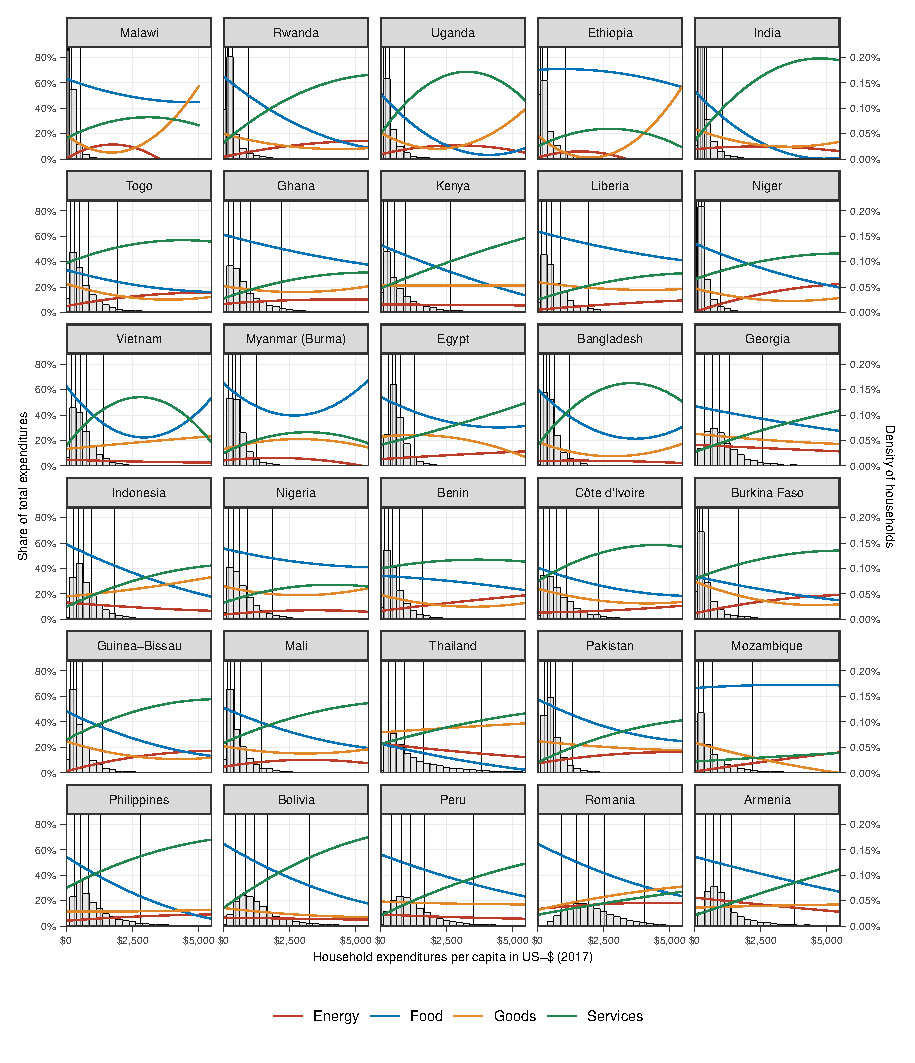
\includegraphics{1_Figures/Analysis_Parametric_Engel_Curves/Parametric_EC_0_A.pdf}
  \caption{Engel curves: expenditure shares over total household expenditures - Part A} \label{fig:Engel_1}
  \begin{subcaption2}
    This figure displays fitted lines for parametric and quadratic Engel curves for each consumption category in 30 countries of our sample. Black vertical lines indicate average household expenditures per capita for each expenditure quintile and country. Grey bars and secondary y-axis indicate the distribution of households.
  \end{subcaption2}
  \end{subfigure}
\end{figure}

\clearpage

\begin{figure}[ht!]\ContinuedFloat
   \begin{subfigure}[b]{\textwidth}
  \centering
  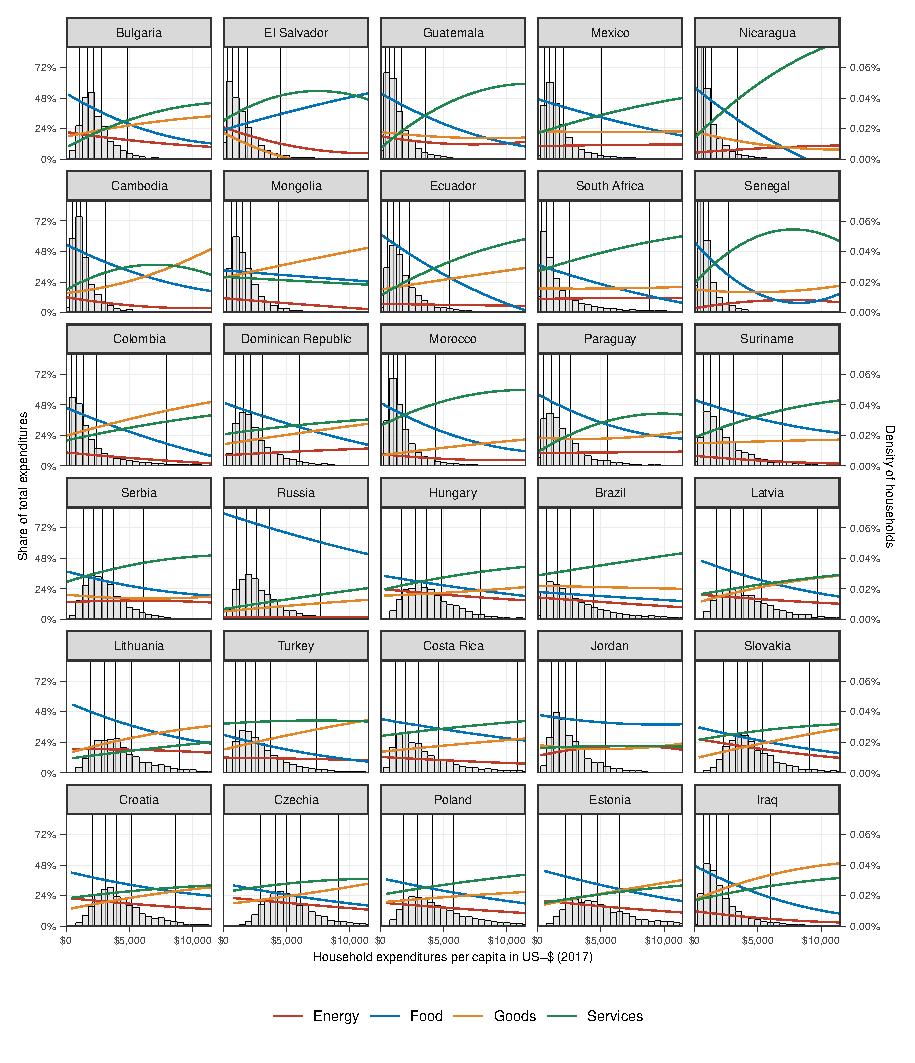
\includegraphics{1_Figures/Analysis_Parametric_Engel_Curves/Parametric_EC_0_B.pdf}
  \caption{Engel curves: expenditure shares over total household expenditures - Part B} \label{fig:Engel_2}
  \begin{subcaption2}
    This figure displays fitted lines for parametric and quadratic Engel curves for each consumption category in 30 countries of our sample. Black vertical lines indicate average household expenditures per capita for each expenditure quintile and country. This figure displays fitted lines for parametric and quadratic Engel curves for each consumption category in 30 countries of our sample. Black vertical lines indicate average household expenditures per capita for each expenditure quintile and country. Grey bars and secondary y-axis indicate the distribution of households.
  \end{subcaption2}
\end{subfigure}
\end{figure}

\clearpage

\begin{figure}[ht!]\ContinuedFloat
   \begin{subfigure}[b]{\textwidth}
  \centering
  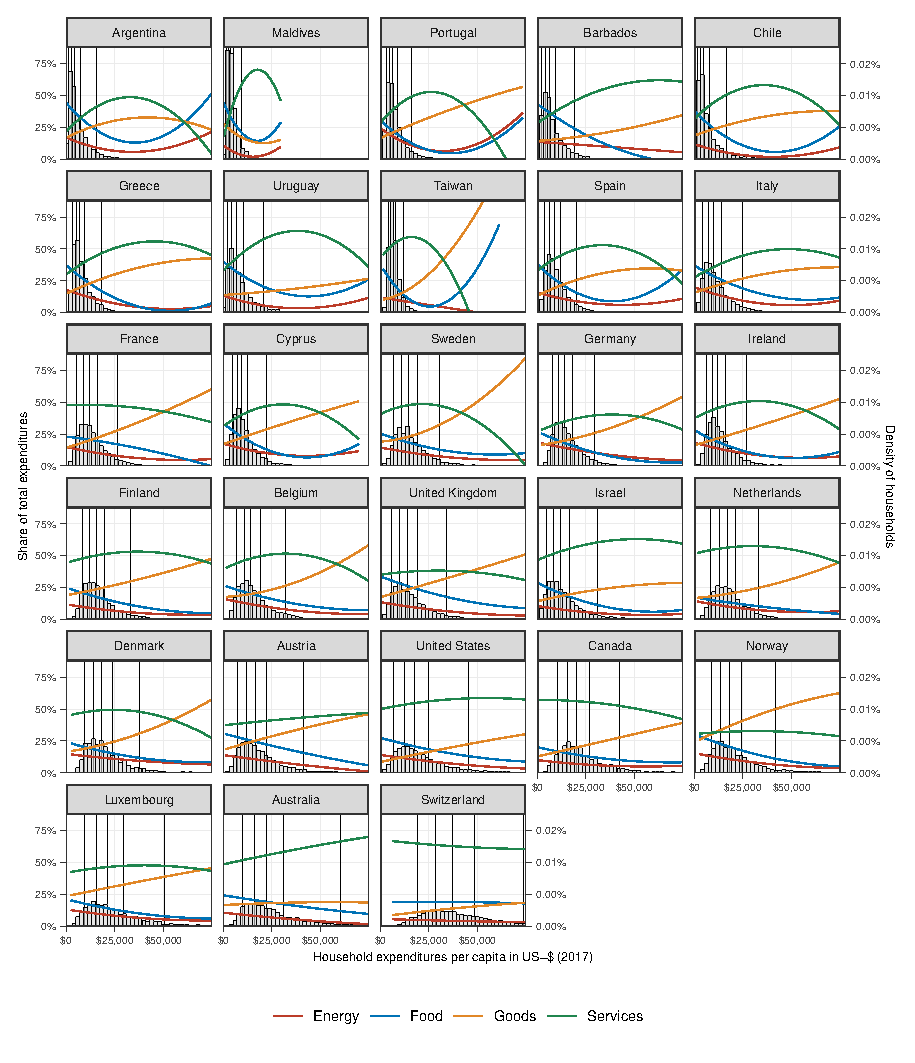
\includegraphics{1_Figures/Analysis_Parametric_Engel_Curves/Parametric_EC_0_C.pdf}
  \caption{Engel curves: expenditure shares over total household expenditures - Part C} \label{fig:Engel_3}
  \begin{subcaption2}
    This figure displays fitted lines for parametric and quadratic Engel curves for each consumption category in 27 countries of our sample. Black vertical lines indicate average household expenditures per capita for each expenditure quintile and country. This figure displays fitted lines for parametric and quadratic Engel curves for each consumption category in 30 countries of our sample. Black vertical lines indicate average household expenditures per capita for each expenditure quintile and country. Grey bars and secondary y-axis indicate the distribution of households.
  \end{subcaption2}
\end{subfigure}
\end{figure}


